\documentclass[final,hyperref={pdfpagelabels=false},professionalfonts,mathserif]{beamer}
\mode<presentation> {\usetheme{Custom}}
\usepackage[scaled]{helvet}
\usepackage{euler}
\usepackage[T1]{fontenc}
% \usepackage[light,math]{iwona}
\usepackage{times}	
\usepackage{amsmath,amsthm, amssymb, latexsym, mathrsfs, amsfonts}
\usepackage{type1cm}
\usepackage{ragged2e} 
% \usepackage{ccaption}
\usepackage{caption, subcaption}
\usepackage{psfrag}
\usepackage{graphicx, float}
% for multiple column output
\usepackage{multicol}
\usepackage{tikz}
\usepackage[authoryear]{natbib}
\usepackage{sidecap}

\usepackage[english]{babel}
\usepackage[utf8]{inputenc}
% \usepackage[size=custom,width=84.1,height=118.9,scale=1.4,debug]{beamerposter}
\usepackage[size=custom,width=84.1,height=114.3,scale=1.2,debug]{beamerposter}
% \useinnertheme{rectangles}
% \setbeamertemplate{itemize items}{\scriptsize\raise1.25pt\hbox{\donotcoloroutermaths$\blacktriangleleft$}}

\DeclareMathOperator*{\argmax}{arg\,max}
\DeclareMathOperator*{\argmin}{arg\,min}

\def\bbE{\mathbb{E}}
\def\bbP{\mathbb{P}}
\def\bfmath#1{\mathchoice
        {\mbox{\boldmath$#1$}}%
        {\mbox{\boldmath$#1$}}%
        {\mbox{\boldmath$\scriptstyle#1$}}%
        {\mbox{\boldmath$\scriptscriptstyle#1$}}}%

\def\bfa{\bfmath{a}}
\def\bfb{\bfmath{b}}
\def\bfo{\bfmath{o}}
\def\cF{\mathcal{F}}
\def\scF{\mathscr{F}}
\newcommand{\inner}[1]{\left\langle #1 \right\rangle}

\def\newblock{\hskip .11em plus .33em minus .07em}
\renewcommand{\raggedright}{\leftskip=0pt \rightskip=0pt plus 0cm}

% \usepackage{stmaryrd} 

%%%%%%%%%%%%%%%%%%%%%%%%%%%%%%%%%%%%%%%%%%%%%%%%%%%%%%%%%%%%%%%%%%%%%
%%             Math Symbols
%%%%%%%%%%%%%%%%%%%%%%%%%%%%%%%%%%%%%%%%%%%%%%%%%%%%%%%%%%%%%%%%%%%%%

%%               Bold Math
\def\mbeta{\boldsymbol{\beta}}

\def\ma{\bm{a}}
\def\mb{\bm{b}}
\def\mc{\bm{c}}
\def\md{\bm{d}}
\def\me{\bm{e}}
\def\mf{\bm{f}}
\def\mg{\bm{g}}
\def\mh{\bm{h}}
\def\mi{\bm{i}}
\def\mj{\bm{j}}
\def\mk{\bm{k}}
\def\ml{\bm{l}}
\def\mm{\bm{m}}
\def\mn{\bm{n}}
\def\mo{\bm{o}}
\def\mp{\bm{p}}
\def\mq{\bm{q}}
\def\mr{\bm{r}}
\def\ms{\bm{s}}
\def\mt{\bm{t}}
%\def\mu{\bm{u}}
\def\bmu{\bm{u}}
\def\mv{\bm{v}}
\def\mw{\bm{w}}
\def\mx{\bm{x}}
\def\my{\bm{y}}
\def\mz{\bm{z}}

\def\mA{\bm{A}}
\def\mB{\bm{B}}
\def\mC{\bm{C}}
\def\mD{\bm{D}}
\def\mE{\bm{E}}
\def\mF{\bm{F}}
\def\mG{\bm{G}}
\def\mH{\bm{H}}
\def\mI{\bm{I}}
\def\mJ{\bm{J}}
\def\mK{\bm{K}}
\def\mI{\bm{I}}
\def\mM{\bm{M}}
\def\mN{\bm{N}}
\def\mO{\bm{O}}
\def\mP{\bm{P}}
\def\mQ{\bm{Q}}
\def\mR{\bm{R}}
\def\mS{\bm{S}}
\def\mT{\bm{T}}
%\def\mu{\bm{u}}
\def\mV{\bm{V}}
\def\mW{\bm{W}}
\def\mX{\bm{X}}
\def\mY{\bm{Y}}
\def\mZ{\bm{Z}}

\def\mini{\text{minimize}}
\def\mm{\bm m}
\def\mone{\mathbf{1}}
\def\mx{\bm x}
\def\mZ{\bm Z}
\def\mA{\bm A}
\def\mB{\bm B}
\def\mS{\bm S}
\def\mC{\bm C}
\def\mI{\bm I}
\def\mT{\bm T}
\def\mK{\bm K}
\def\mG{\bm G}
\def\mX{\bm X}
\def\mY{\bm Y}
\def\mM{\bm M}
\def\mSigma{\bm \Sigma}
\def\mOmega{\bm \Omega}

\def\nmA{\bm{\widetilde A}}
\def\nmB{\bm{\widetilde B}}
\def\nmC{\bm{\widetilde C}}
\def\nmD{\bm{\widetilde D}}
\def\nmE{\bm{\widetilde E}}
\def\nmF{\bm{\widetilde F}}
\def\nmG{\bm{\widetilde G}}
\def\nmH{\bm{\widetilde H}}
\def\nmI{\bm{\widetilde I}}
\def\nmJ{\bm{\widetilde J}}
\def\nmK{\bm{\widetilde K}}
\def\nmL{\bm{\widetilde L}}
\def\nmM{\bm{\widetilde M}}
\def\nmN{\bm{\widetilde N}}
\def\nmO{\bm{\widetilde O}}
\def\nmP{\bm{\widetilde P}}
\def\nmQ{\bm{\widetilde Q}}
\def\nmR{\bm{\widetilde R}}
\def\nmS{\bm{\widetilde S}}
\def\nmT{\bm{\widetilde T}}
\def\nmU{\bm{\widetilde U}}
\def\nmV{\bm{\widetilde V}}
\def\nmW{\bm{\widetilde W}}
\def\nmX{\bm{\widetilde X}}
\def\nmY{\bm{\widetilde Y}}
\def\nmZ{\bm{\widetilde Z}}
\def\nmSig{\bm{\widetilde \Sigma}}

\def\nA{\mathcal{\widetilde A}}
\def\nB{\mathcal{\widetilde B}}
\def\nC{\mathcal{\widetilde C}}
\def\nD{\mathcal{\widetilde D}}
\def\nE{\mathcal{\widetilde E}}
\def\nF{\mathcal{\widetilde F}}
\def\nG{\mathcal{\widetilde G}}
\def\nH{\mathcal{\widetilde H}}
\def\nI{\mathcal{\widetilde I}}
\def\nJ{\mathcal{\widetilde J}}
\def\nK{\mathcal{\widetilde K}}
\def\nL{\mathcal{\widetilde L}}
\def\nM{\mathcal{\widetilde M}}
\def\nN{\mathcal{\widetilde N}}
\def\nO{\mathcal{\widetilde O}}
\def\nP{\mathcal{\widetilde P}}
\def\nQ{\mathcal{\widetilde Q}}
\def\nR{\mathcal{\widetilde R}}
\def\nS{\mathcal{\widetilde S}}
\def\nT{\mathcal{\widetilde T}}
\def\nU{\mathcal{\widetilde U}}
\def\nV{\mathcal{\widetilde V}}
\def\nW{\mathcal{\widetilde W}}
\def\nX{\mathcal{\widetilde X}}
\def\nY{\mathcal{\widetilde Y}}
\def\nZ{\mathcal{\widetilde Z}}




\def\tZ{\mathcal{Z}}
\def\tA{\mathcal{A}}
\def\tB{\mathcal{B}}
\def\tC{\mathcal{C}}
\def\tD{\mathcal{D}}
\def\tE{\mathcal{E}}
\def\tF{\mathcal{F}}
\def\tG{\mathcal{G}}
\def\tH{\mathcal{H}}
\def\tI{\mathcal{I}}
\def\tJ{\mathcal{J}}
\def\tK{\mathcal{K}}
\def\tL{\mathcal{L}}
\def\tM{\mathcal{M}}
\def\tN{\mathcal{N}}
\def\tO{\mathcal{O}}
\def\tP{\mathcal{P}}
\def\tQ{\mathcal{Q}}
\def\tR{\mathcal{R}}
\def\tS{\mathcal{S}}
\def\tT{\mathcal{T}}
\def\tU{\mathcal{U}}
\def\tV{\mathcal{V}}
\def\tW{\mathcal{W}}
\def\tX{\mathcal{X}}
\def\tY{\mathcal{Y}}
\def\tZ{\mathcal{Z}}
\def\trueB{\mathcal{B}_{\text{true}}}
\def\trueT{\Theta_{\text{true}}}
\def\trueM{\mM_{k,\text{true}}}
\def\trueC{\tC_{\text{true}}}

\def\fixme#1#2{\textbf{[FIXME (#1): #2]}}
\def\entry#1{\llbracket #1 \rrbracket}
\def\est{\bm{\widehat u}_1} %% first eigenvector estimate
\def\estv{\widehat \lambda_1}%% first eigenvalue estimate
\def\esti{\bm{\widehat u}_i}%% i-th eigenvector estimate
\def\estvi{\widehat \lambda_i}%% i-th eigenvalue estiamte
\def\true{\bm{u}_1} %% first true eigenvector
\def\truev{\lambda_1}%% first true eigenvalue
\def\ls#1{\mathcal{#1}} %% space
\def\ntensor{\mathcal{\widetilde T}} %% noisy tensor
\def\nHOSVD{\mathcal{\widetilde T}_{(12)(3\ldots k)}} %% noisy two-mode HOSVD
\def\tensor#1{\mathcal{#1}} %% tensor
\def\entry#1{\llbracket #1 \rrbracket}
\def\bigEntry#1{\Big\llbracket #1 \Big\rrbracket}
\def\noisetensor{\mathcal{\widetilde E}} %% noise tensor
\def\noiseHOSVD{\mathcal{\widetilde E}_{(12)(3\ldots k)}} % noise matrix unfolding
\def\eqdef{\stackrel{\text{\tiny \rm def}}{=}} 
\def\Vec{\operatorname{Vec}}
\def\Spanspace{\operatorname{Span}}
\def\Loss{\operatorname{Loss}}
\def\bbR{\mathbb{R}}

\newcommand{\matr}[1]{\bm{#1}}
\newcommand{\norm}[1]{\left\lVert#1\right\rVert_2}
\newcommand{\onenorm}[1]{\left\lVert#1\right\rVert_1}
\newcommand{\zeronorm}[1]{\left\lVert#1\right\rVert_0}
\newcommand{\mnorm}[1]{\left\lVert#1\right\rVert_\text{max}}
\newcommand{\Fnorm}[1]{\left\lVert#1\right\rVert_F}
\newcommand{\nnorm}[1]{\left\lVert#1\right\rVert_*}

\newcommand{\zeronormSize}[2]{#1\lVert#2#1\rVert_0}
\newcommand{\nnormSize}[2]{#1\lVert#2#1\rVert_*}
\newcommand{\vnormSize}[2]{#1\lVert#2#1\rVert_2}
\newcommand{\normSize}[2]{#1\lVert#2#1\rVert}
\newcommand{\snormSize}[2]{#1\lVert#2#1\rVert_\sigma}
\newcommand{\FnormSize}[2]{#1\lVert#2#1\rVert_F} 
\newcommand{\mnormSize}[2]{#1\lVert#2#1\rVert_\text{max}} 

\DeclareMathOperator*{\argmin}{arg\,min}
\DeclareMathOperator*{\argmax}{arg\,max}
\DeclareMathOperator*{\maximize}{maximize}

\newcommand{\suppfref}[1]{{Supplementary Figure~\ref{#1}}}
\newcommand{\supptref}[1]{{Supplementary Table~\ref{#1}}}
\def\sref#1{Section~\ref{#1}}
\setbeamercolor{caption name}{fg=black}
\setbeamercolor{caption body}{fg=black}
\setbeamertemplate{itemize items}[triangle]
\setlength{\leftmargini}{1.3cm}
%%%%%%%%%%%%%%%%%%%%%%%%%%%%%%%%%%%%%%%%%%%%%%%%%%%%%%%%%%%%%%%%%%%%%%%%%%%%%%%%%5
\graphicspath{{graphics/}}
\title{Efficient inference of population size changes and mutation rates\\ using the site frequency spectrum from large samples}
\author{Anand Bhaskar${}^1$ and Yun S. Song${}^{1,2}$}
\institute{${}^{1}$Computer Science Division and ${}^{2}$Department of Statistics, University of California, Berkeley}
% \date{June 8, 2013}
%%%%%%%%%%%%%%%%%%%%%%%%%%%%%%%%%%%%%%%%%%%%%%%%%%%%%%%%%%%%%%%%%%%%%%%%%%%%%%%%%5
\begin{document}
\begin{frame}[fragile]
\vspace{-1cm}
\begin{columns}[t]
	\begin{column}{.495\linewidth}
		\begin{block}{\large Motivation}\justifying 
			\begin{columns}[T]
			\begin{column}{.97\linewidth}
                \vspace{-0.5cm}
				Null models in population genetics are used for, among many other things,
				\begin{itemize}
					\item Finding genomic regions under selection
					\item Genome-wide association studies
					\item Reconstructing demography
					\item Forensic applications
					% \vspace{1mm}
					% \quad{}\vdots
				\end{itemize}				
				Commonly used null model assumptions:
				\begin{itemize}
					\item Constant effective population size
					\item Constant mutation rate across loci
					\item No population substructure
				\end{itemize}
				Several recent large-sample datasets have found an excess of rare variants
				compared to predictions from previously inferred demographic models
				\begin{itemize}
					\item \citet{coventry:2010} - 13,715 individuals at 2 genes
					\item \citet{tennessen:2012} - 2,440 individuals at 15,585 genes 
					\item \citet{nelson:2012} - 14,002 individuals at 202 genes
				\end{itemize}		
				\vspace{5pt}
				\centerline{
				% \vspace{5pt}
				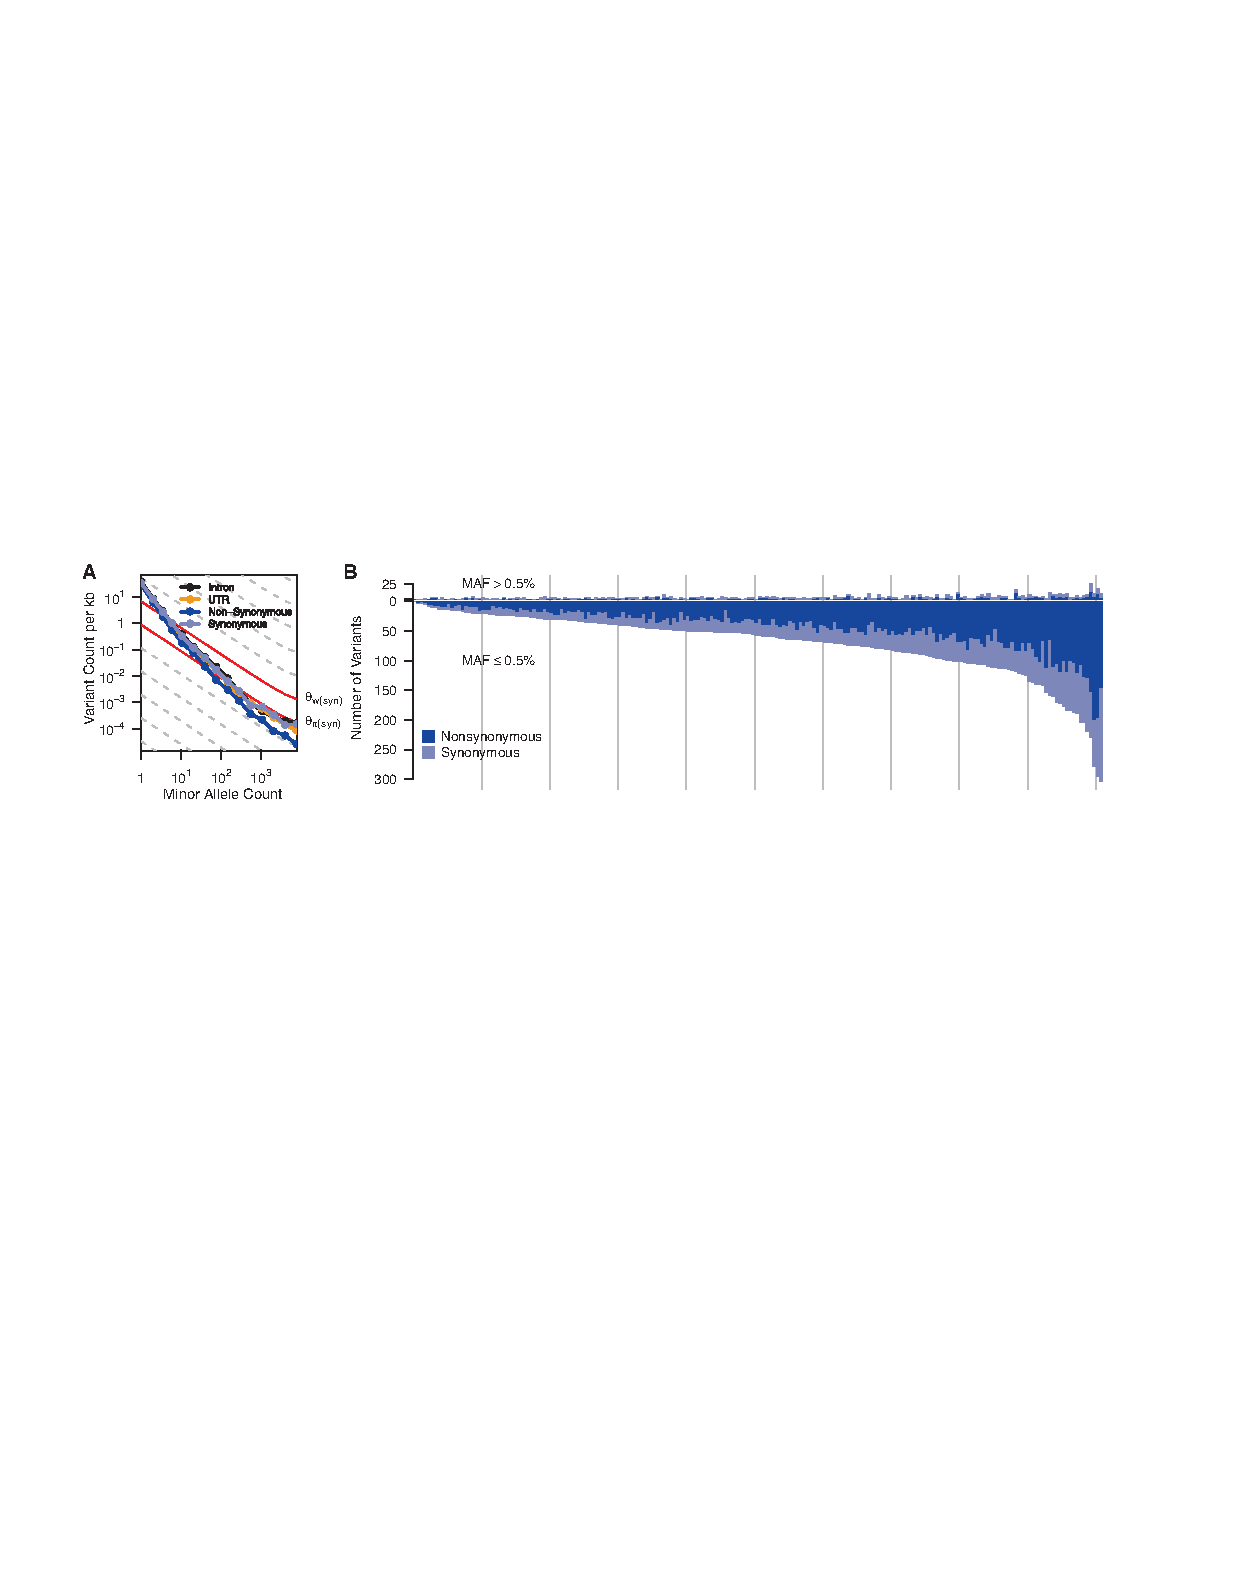
\includegraphics[width=14in]{figs/Nelson_variants_by_frequency} \\
				}
				(Figure from \citeauthor{nelson:2012}, 2012) \\
				% Similar observations made by \citet{coventry:2010, tennessen:2012}.
				Recent exponential population growth can explain the abundance of rare variants \\% \citep{keinan:2012} \\
				Need large sample sizes of tens of thousands of individuals to infer such growth
			\end{column}
			\end{columns}
		\end{block}

		\begin{block}{\large Problem} \justifying
			\begin{columns}[T]
			\begin{column}{.97\linewidth}
			    % \setlength{\columnsep}{2cm}
                \vspace{-0.5cm}
				Data: Sample of $n$ haplotypes at several unlinked loci \\
				Summarize the data by the site frequency spectrum (SFS) at each locus\\ $\bfo = (o_1, o_2, \ldots, o_{n-1})$, where $o_i$ = number of SNVs with $i$ copies of the derived allele (can use the folded SFS if the ancestral allele is not known) \\
				% Model: Kingman's coalescent with infinite-sites mutation \\
				Goal: Given SFS from a \emph{large sample} at many loci, infer \emph{historical population size changes} \\
				Previous approaches:
				\begin{itemize}
					\item Full likelihood approaches based on the sequentially Markovian coalescent (\citeauthor{li:2011}, 2011; \citeauthor{sheehan:2013}, 2012). Cannot scale to large sample sizes needed to infer recent population expansion events
					\item Monte-Carlo coalescent-based methods for the SFS \citep{coventry:2010}. Unsuitable for gradient-based optimization, requiring grid search for the population size changes and mutation rates
					\item Diffusion-theoretic methods for the SFS. Handle rich class of demographic models, but can suffer from discretization accuracy issues, especially for large population sizes
				\end{itemize}
			\end{column}
			\end{columns}
		\end{block}


        \begin{block}{\large Our method} \justifying
	        \begin{columns}[T] 
            \begin{column}{.97\linewidth}
	   		% \setlength{\columnsep}{2cm}
	   		    \vspace{-0.5cm}
				Population size function $\{ N(t), t \geq 0 \}$ is not identifiable in general from SFS data. \\
				Restrict attention to population size functions $N(t)$ in a restricted family of functions $\cF$. \\
				We consider the family $\cF$ of piecewise exponential functions with $M$ pieces.
				\begin{itemize}
					\item Time intervals for pieces $[t_i, t_{i+1})$, $0 \leq i < M$, $t_0 := 0, t_M := \infty$
					\item Population growth rates $\beta_{i+1}$ in piece $[t_i, t_{i+1})$, $0 \leq i < M - 1$
					\item $\beta_M := 0$ (constant ancestral population size)
					\item $N(t) = N(t_i) \exp(- \beta_{i+1} (t - t_i))$ for $t \in [t_i, t_{i+1})$
				\end{itemize}
				This family of functions can capture arbitrary number of epochs of exponential population growth, bottlenecks, and intervals of constant population size. \\
			    For a sample of size $n$ and demographic model $\Phi \in \cF$, define:
			    \begin{itemize}
					\item $T^{\Phi}_{n,i}$ -- waiting time in the coalescent while there are $i$ lineages given that there are $n$ lineages at the current time $t = 0$, $2 \leq i \leq n$
			        \item $\tau^{\Phi}_{n,i}$ -- total length of edges subtending $i$ leaves in coalescent tree, $1 \leq i \leq n-1$
			        \item $L^{\Phi}_n$ -- total length of edges in coalescent tree
			    \end{itemize}
				Mutations on edges subtending $i$ lineages contribute to the $i^{th}$ entry of the SFS.\\
				Under the Poisson random field approximation of sites being completely unlinked within a locus, the log-likelihood can be written as,
				\begin{align*}
					\log \bbP(\bfo \mid \Phi, \theta) &= \sum_{i=1}^{n-1} o_i \left(\log \bbE\left[\tau^{\Phi}_{n,i}\right] + \log\theta \right) - \frac{\theta}{2} \bbE\left[L^{\Phi}_{n}\right]
				\end{align*}
				MLE for $\theta$ is $\theta^*$, given by a generalization of Watterson's estimator to variable population models,
				\begin{align*}
					\theta^* = \frac{2 \sum_{i=1}^{n-1} o_i}{\bbE\left[L^{\Phi}_{n}\right]}
				\end{align*}
				% $\bbE[o_i] = {\theta \over 2} \bbE[\tau_{n,i}]$
				MLE for $\Phi$ is $\Phi^*$ which minimizes the KL-divergence of the expected SFS from the observed SFS,
				\begin{align*}
					\Phi^* = \argmin_{\Phi} \textrm{KL}\left( \left. \frac{\bfo}{\lvert \bfo \rvert} \, \right\| \frac{\bbE\left[\bfmath{\tau}^{\Phi}_n\right]}{\bbE\left[L^{\Phi}_n\right]} \right)
				\end{align*}
				Can compute $\bbE\left[\tau^{\Phi}_{n,i}\right]$ and $\bbE\left[L^{\Phi}_n\right]$ exactly and efficiently for models $\Phi \in \cF$ using analytical theory of the SFS. \\
				Gradient of log-likelihood with respect to model parameters can be calculated using automatic differentiation.
		    \end{column} 
	        \end{columns} 
        \end{block}
        
	\end{column}


	\begin{column}{.495\linewidth}
		
		
		\begin{block}{\large Computational details}
			\begin{columns}[T]
			\begin{column}{.97\linewidth}
			\vspace{-0.5cm}
			\citet{polanski:2003-1} showed that for arbitrary population size functions $N(t)$ and mutation rate $\theta$,
			\vspace{-0.8cm}
			\begin{align*}
				\bbE[\tau_{n,i}] &= \frac{\theta}{2} \sum_{k=2}^{n} a_{n,i,k} \bbE[T_{k,k}]	\\
				\bbE[L_n] &= \frac{\theta}{2} \sum_{k=2}^{n} b_{n,k} \bbE[T_{k,k}],
			\end{align*}
			where $a_{n,i,k}$ and $b_{n,k}$ are \emph{universal coefficients} that do not depend on $N(t)$. All the dependence on the population model is captured in $\bbE[T_{k,k}]$,
			\begin{align*}
				\bbE[T_{k,k}] = \int_0^{\infty} t ~\frac{\binom{k}{2}}{N(t)} \exp \left( - \int_0^t \frac{\binom{k}{2}}{N(s)} ds \right) dt
			\end{align*}
			Each coefficient $a_{n,i,k}$ and $b_{n,k}$ can be computed in $O(1)$ time by dynamic programming. \\
			For functions $N(t)$ in our family of models $\cF$, the integral in $\bbE[T_{k,k}]$ can be solved in terms of exponential functions and the exponential integral special function $\textrm{Ei}(x)$, and can be computed in $O(M)$ time.
			\end{column}
			\end{columns}
		\end{block}

		\begin{block}{\large Evaluation} \justifying 
			\begin{columns}[T]
        	\begin{column}{0.97\linewidth}
                % \vspace{-0.5cm}
				\begin{figure}[H]
				    % \centering
				  \begin{subfigure}[b]{0.48\linewidth}
				      \centering
				      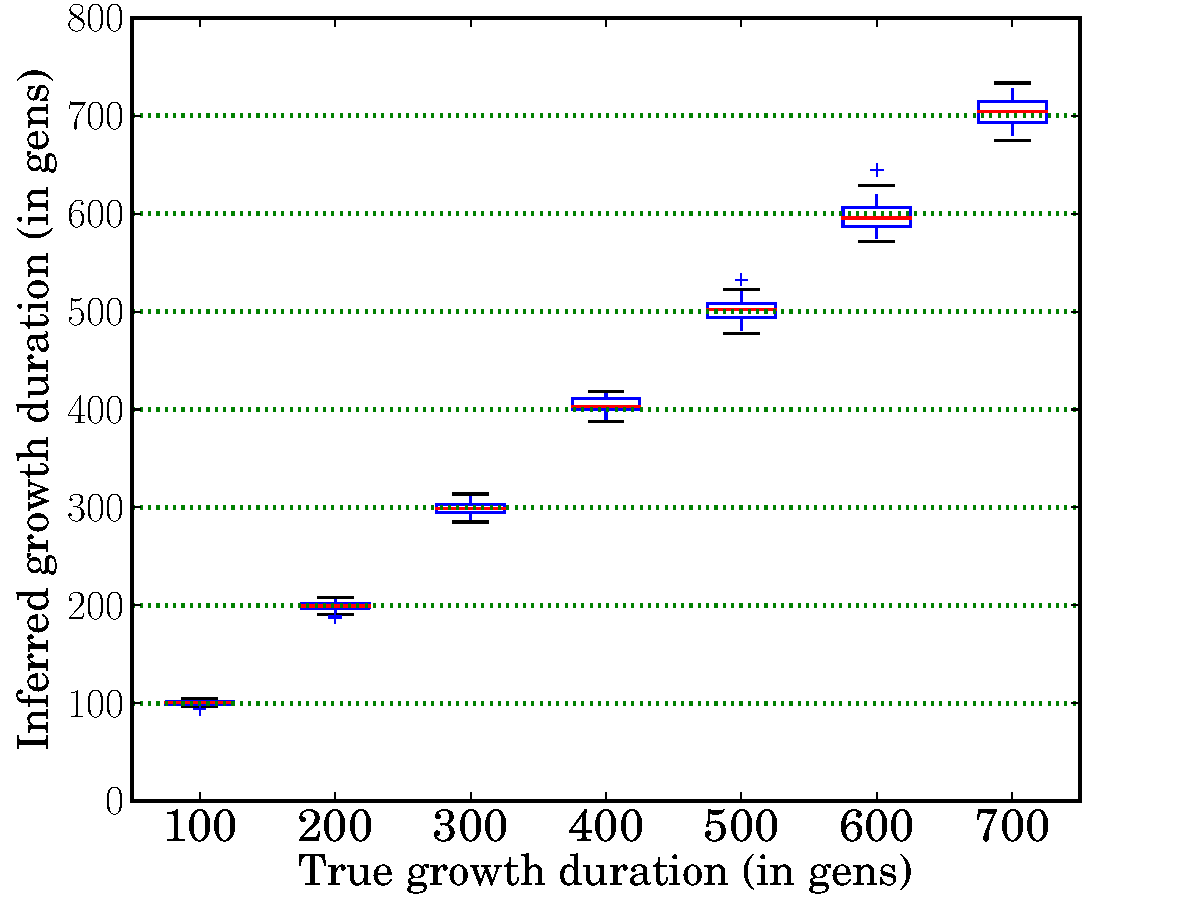
\includegraphics[type=pdf,ext=.pdf,read=.pdf,trim=0 0 0 1cm]{figs/our_method_nomad_allRuns_rho0.4_maxb18_boxPlotTOnsets}
				        \caption{}
				      \label{fig:inferred_params_1epoch_duration}
				    \end{subfigure}
				  \begin{subfigure}[b]{0.48\linewidth}
				      \centering
				      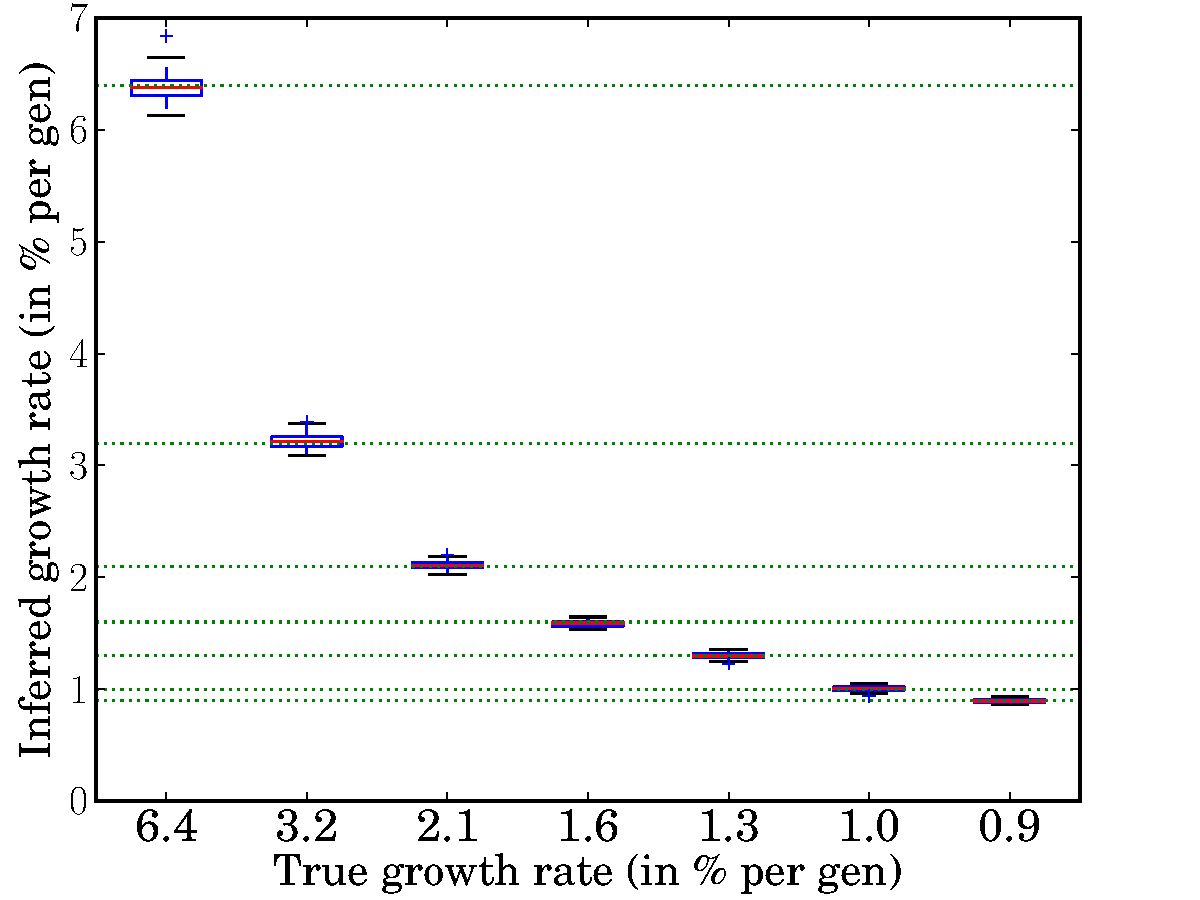
\includegraphics[type=pdf,ext=.pdf,read=.pdf,trim=0 0 0 1cm]{figs/our_method_nomad_allRuns_rho0.4_maxb18_boxPlotRs}
				        \caption{}
				      \label{fig:inferred_params_1epoch_growth_rate}
				    \end{subfigure}
				    \label{fig:inferred_params_1epoch}
				    \caption{
				    Box plots of the inferred (\protect\subref{fig:inferred_params_1epoch_duration}) duration and (\protect\subref{fig:inferred_params_1epoch_growth_rate}) rate of exponential growth for 100 simulated datasets with 10,000 individuals at 200 loci for 7 population expansion scenarios. The dotted green lines indicate the true values for the inferred parameters. % Figure (\subref{fig:inferred_mutation_rates}) shows the inferred mutation rates at a random subset of 15 loci for 100 simulated datasets, where the loci are sorted by their true mutation rates.
				    }
				\end{figure}

				\begin{figure}[H]
				    % \centering
				  \begin{subfigure}[b]{0.48\linewidth}
				      \centering
				      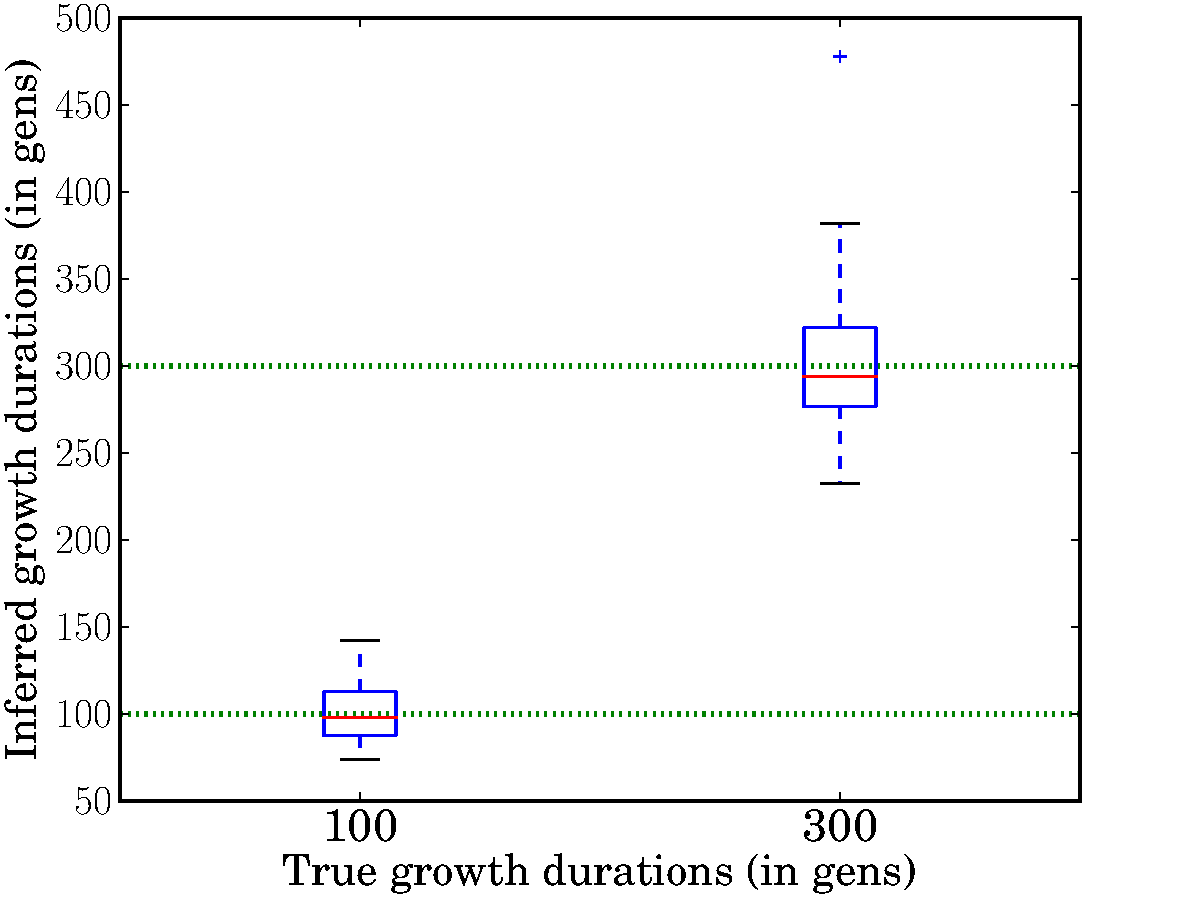
\includegraphics[type=pdf,ext=.pdf,read=.pdf]{figs/our_method_2epoch_r4t100r1t300_rho0.4_n20000_boxPlotTOnsets}
				        \caption{}
				      \label{fig:inferred_params_2epoch_duration}
				    \end{subfigure}
				  \begin{subfigure}[b]{0.48\linewidth}
				      \centering
				      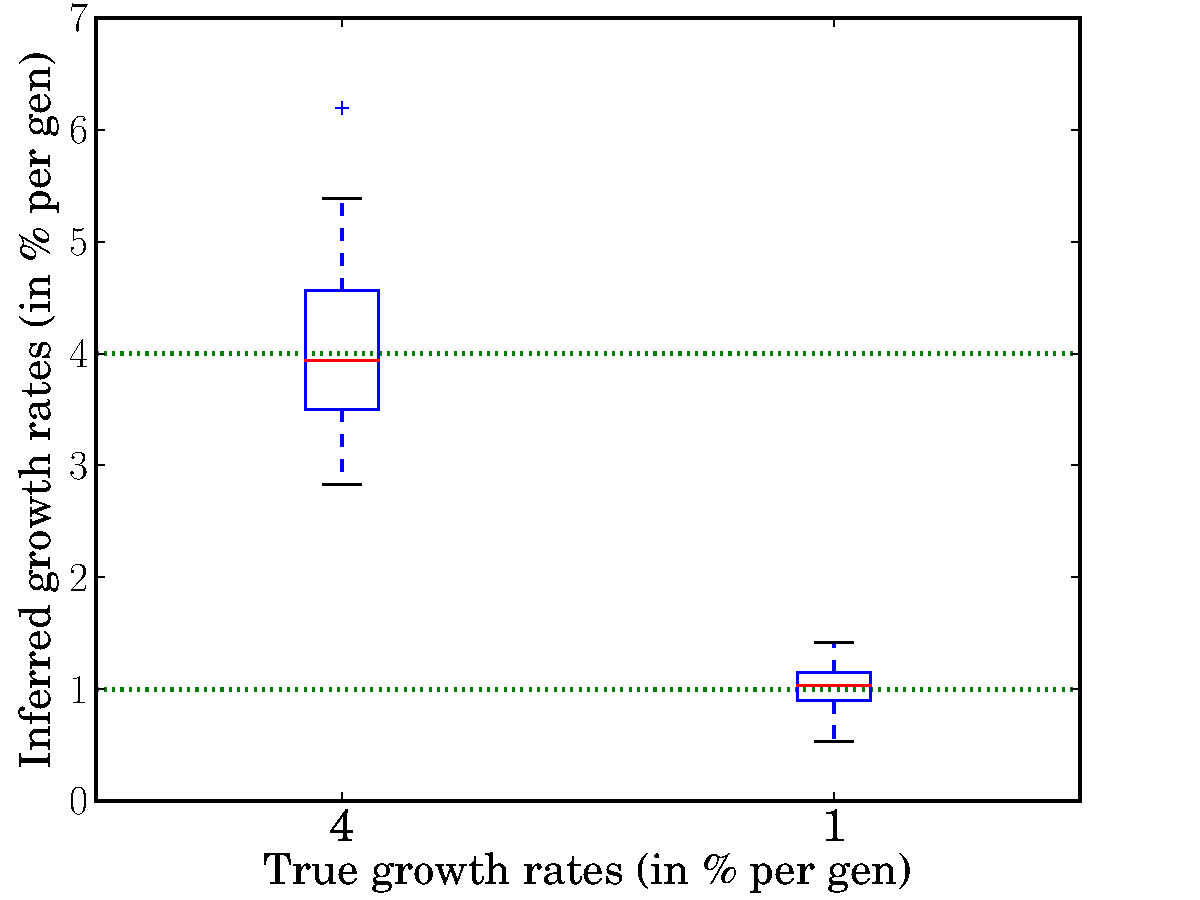
\includegraphics[type=pdf,ext=.pdf,read=.pdf]{figs/our_method_2epoch_r4t100r1t300_rho0.4_n20000_boxPlotRs}
				        \caption{}
				      \label{fig:inferred_params_2epoch_growth_rate}
				    \end{subfigure}
				    \label{fig:inferred_params_2epochs}
				    \caption{
				    Box plots of the inferred (\protect\subref{fig:inferred_params_2epoch_duration}) durations and (\protect\subref{fig:inferred_params_2epoch_growth_rate}) exponential growth rates for 50 simulated datasets with 10,000 individuals at 200 loci, with 2 epochs of recent exponential growth. The dotted green lines indicate the true values for the inferred parameters. % Figure (\subref{fig:inferred_mutation_rates}) shows the inferred mutation rates at a random subset of 15 loci for 100 simulated datasets, where the loci are sorted by their true mutation rates.
				    }
				\end{figure}

				% \begin{figure}[H]
				% \floatbox[{\capbeside\thisfloatsetup{capbesideposition={right,top},capbesidewidth=4cm}}]{figure}[\FBwidth]
				% {\caption{A test figure with its caption side by side}\label{fig:test}}
				% {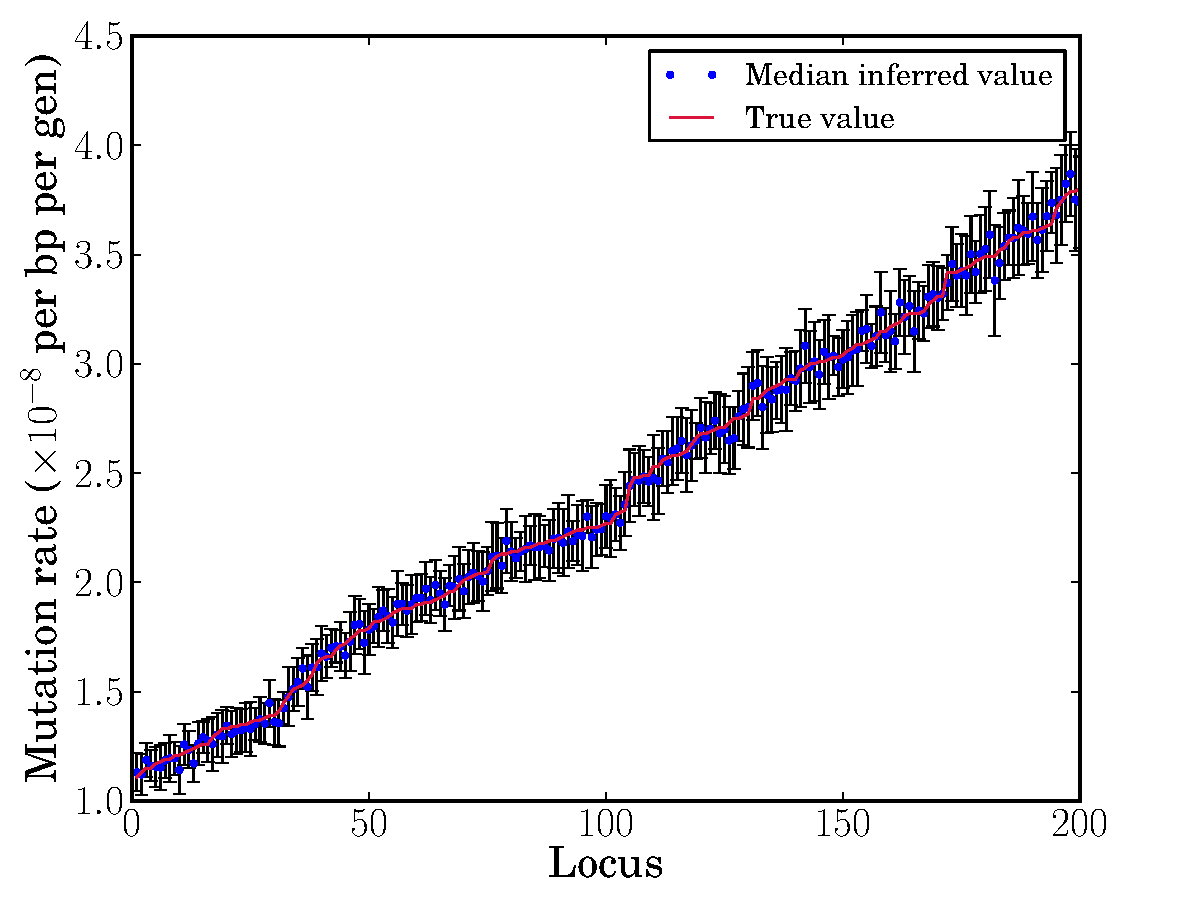
\includegraphics[width=0.45\linewidth,type=pdf,ext=.pdf,read=.pdf]{figs/our_method_nomad_t100_r6.4_rho0.4_maxb18_plotMus}}
				% \end{figure}

				\vspace{-1cm}
				\begin{columns}
				\begin{column}{0.6\linewidth}				
				\begin{figure}[H]
					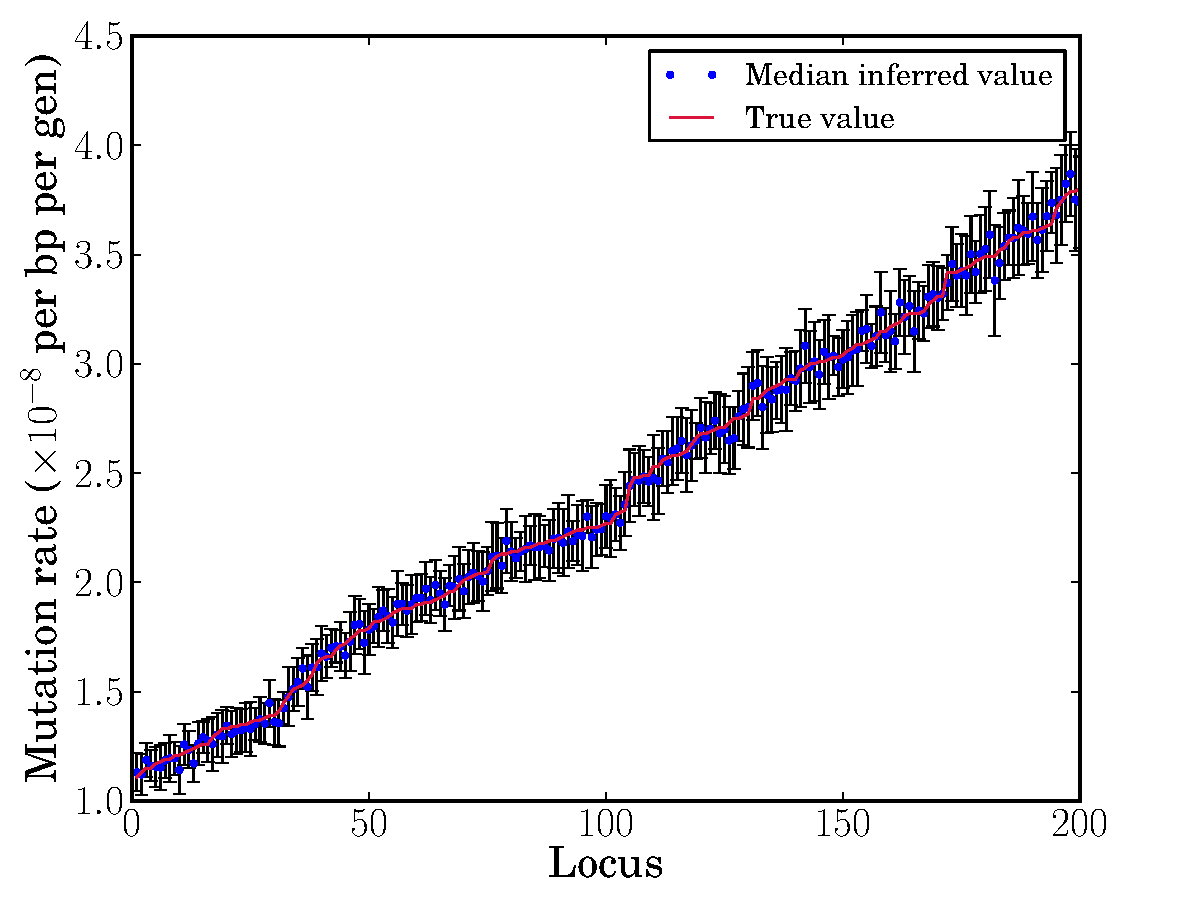
\includegraphics[width=0.99\linewidth,type=pdf,ext=.pdf,read=.pdf]{figs/our_method_nomad_t100_r6.4_rho0.4_maxb18_plotMus}
				\end{figure}
				\end{column}
				\hspace{-3cm}
				\begin{column}[c]{0.38\linewidth}
				Inferred mutation rates at 200 loci with a recent epoch of exponential growth of 100 generations at 6.4\% per generation. The loci are sorted by their true mutation rates.
				\end{column}
				\end{columns}
				\vspace{-0.5cm}
				
				% \begin{figure}
				% 	% \centering
				% 	\parbox[b]{.55\linewidth}{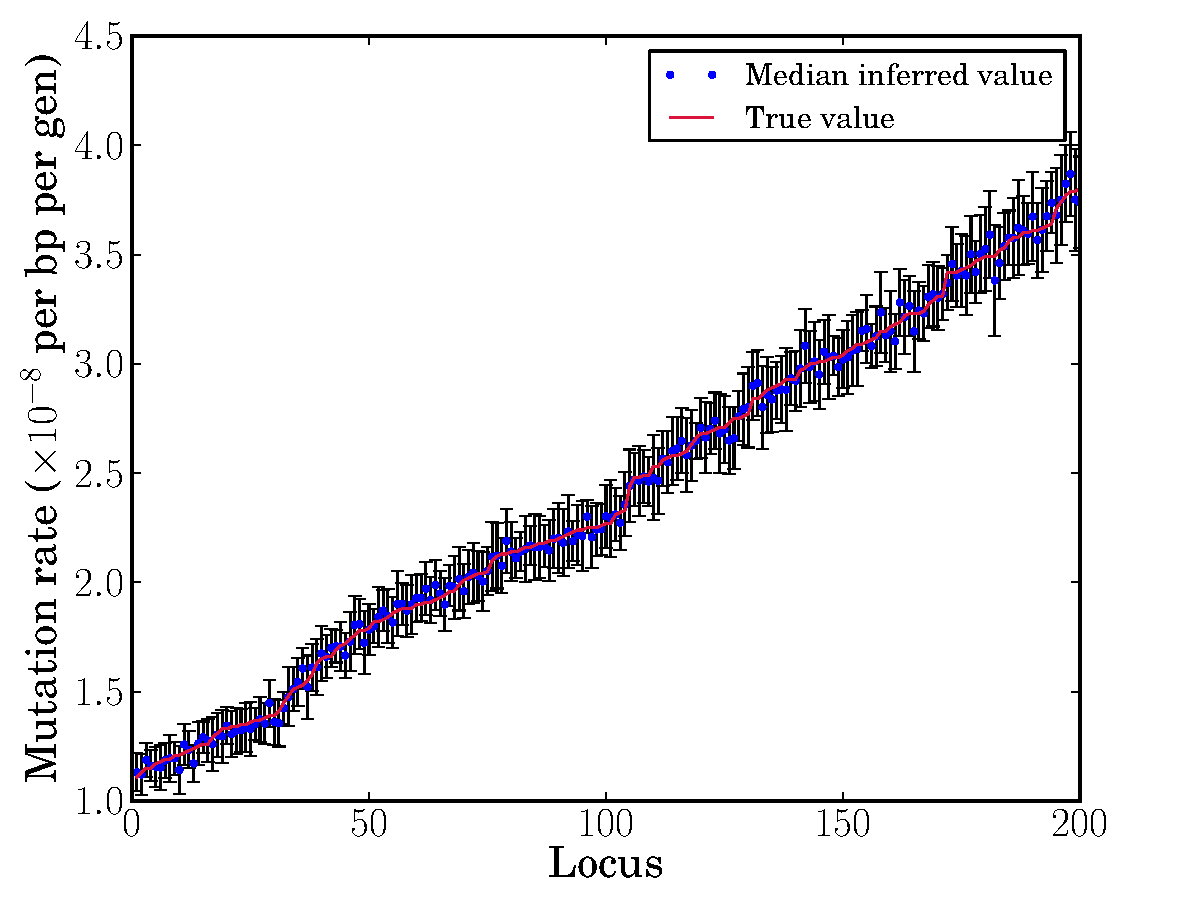
\includegraphics[width=0.99\linewidth,type=pdf,ext=.pdf,read=.pdf]{figs/our_method_nomad_t100_r6.4_rho0.4_maxb18_plotMus}}\hfill
				% 	\parbox[t]{.41\linewidth}{
				% 		\caption{Inferred mutation rates at 200 loci with a recent epoch of exponential growth lasting 100 generations at 6.4\% per generation. The loci are sorted by their true mutation rates.}
				% 		\label{fig:inferred_mutation_rates}
				% 	}
				% \end{figure}

				% \begin{columns}
				% \begin{column}{0.33\linewidth}				
				% \begin{figure}[H]
				% 	\centering
				% 	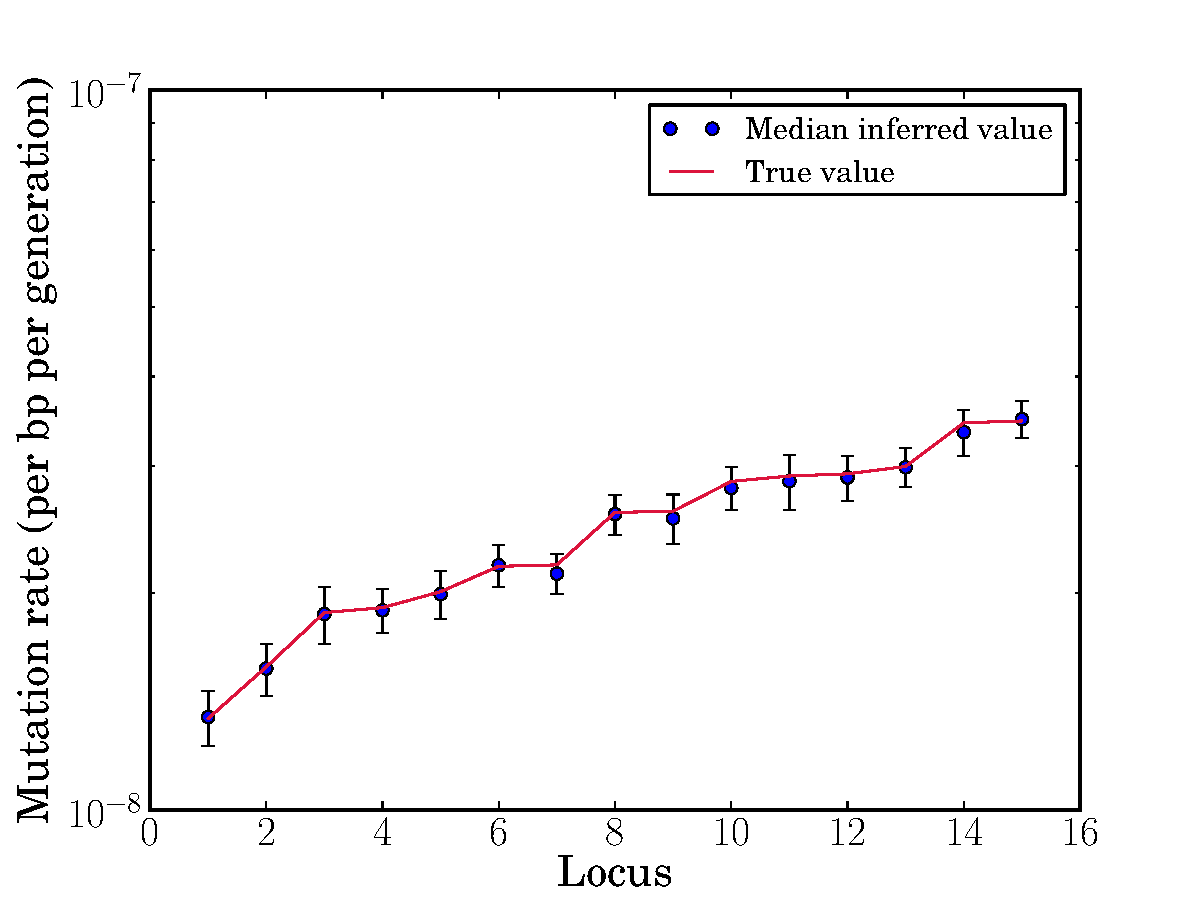
\includegraphics[type=pdf,ext=.pdf,read=.pdf,trim=0 0 0 2.5cm]{figs/our_method_sdbox_t100_r6.4_rho0.4_maxb18_plotMus}
				% 	\label{fig:inferred_mutation_rates}
				% 	\caption{
				% 	Inferred mutation rates at a random subset of 15 loci for 100 simulated datasets with a recent epoch of exponential growth lasting 100 generations at 6.4\% per generation. The loci are sorted by their true mutation rates.
				% 	}
				% \end{figure}
				% \end{column}
				%                 \begin{column}{0.66\linewidth}                
				% 	\begin{figure}[H]
				% 	    % \centering
				% 	  \begin{subfigure}[b]{0.33\linewidth}
				% 	      \centering
				% 	      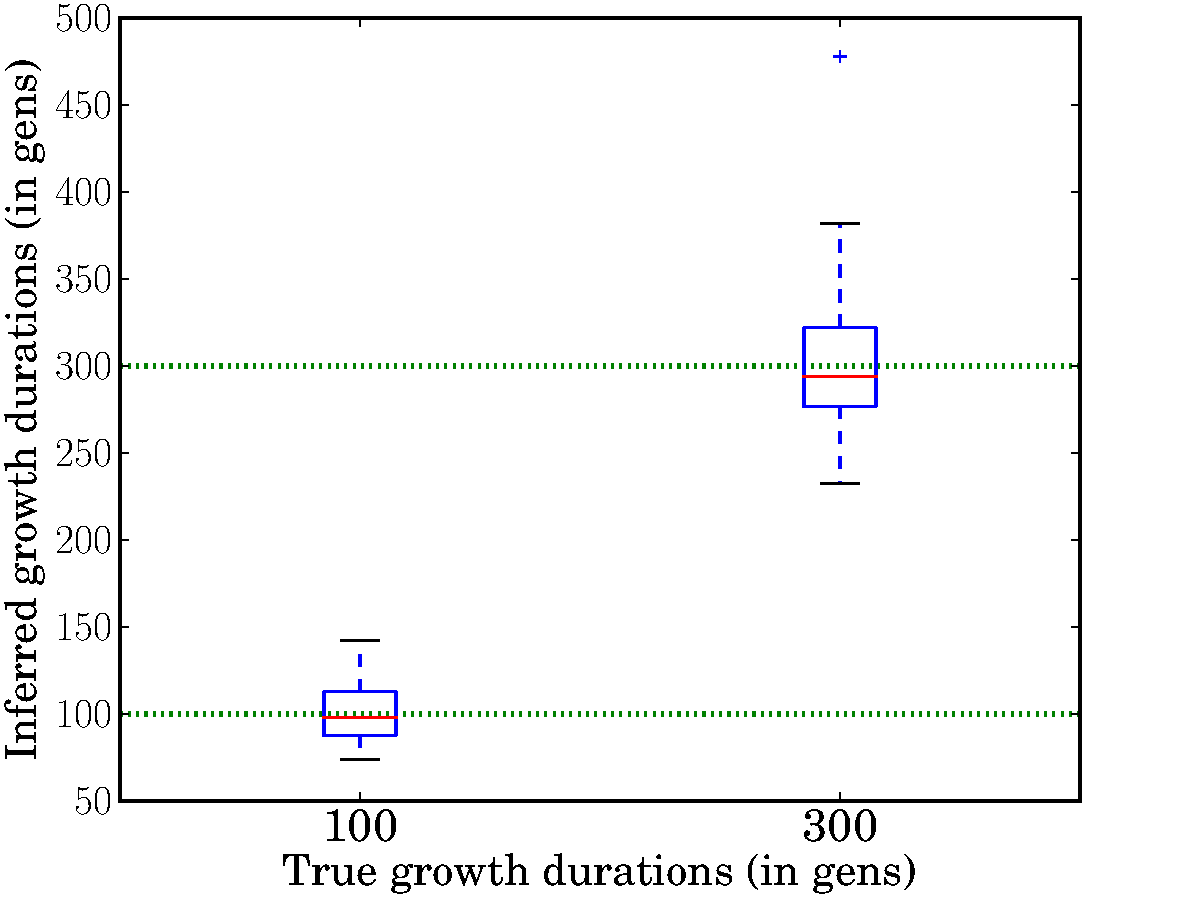
\includegraphics[type=pdf,ext=.pdf,read=.pdf,trim=0 0 0 1cm]{figs/our_method_2epoch_r4t100r1t300_rho0.4_n20000_boxPlotTOnsets}
				% 	        \caption{}
				% 	      \label{fig:inferred_params_1epoch_duration}
				% 	    \end{subfigure}
				% 	  \begin{subfigure}[b]{0.33\linewidth}
				% 	      \centering
				% 	      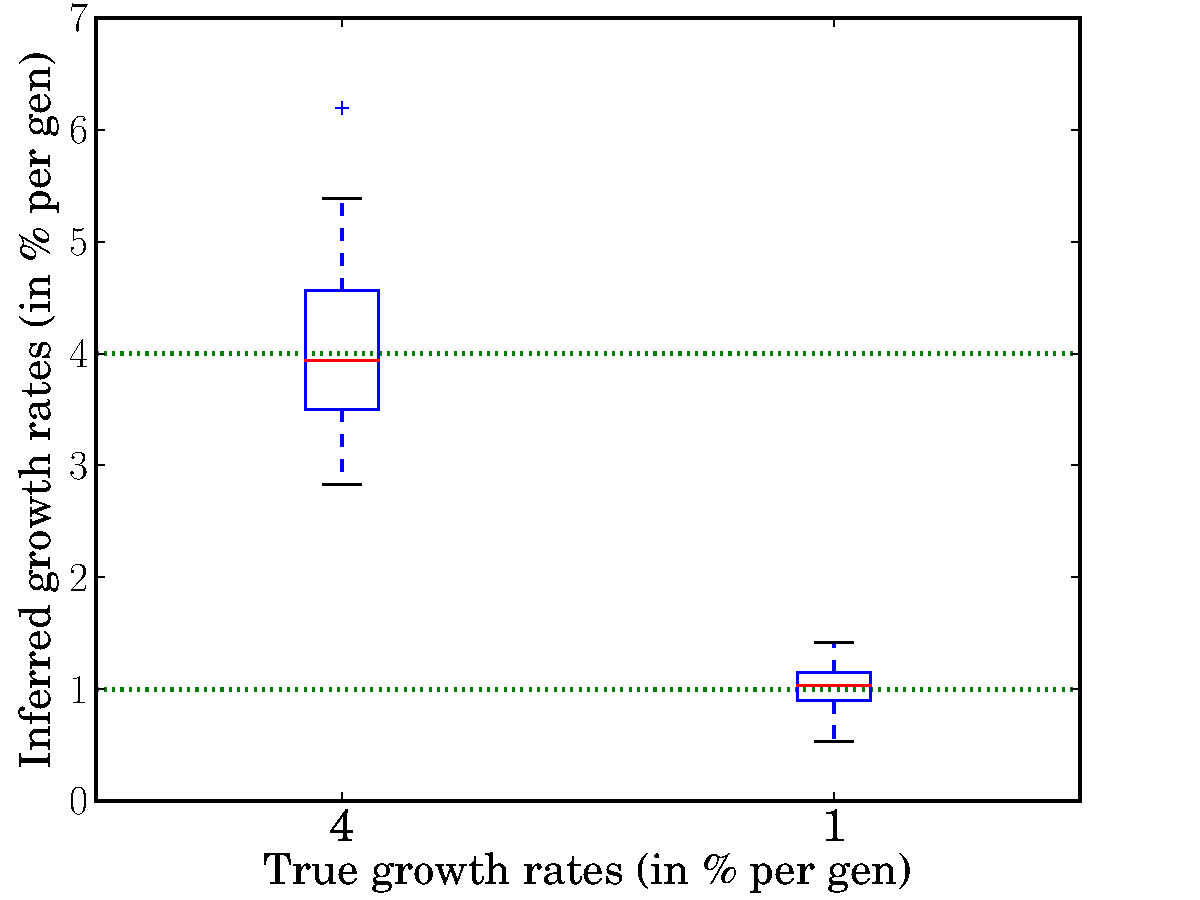
\includegraphics[type=pdf,ext=.pdf,read=.pdf,trim=0 0 0 1cm]{figs/our_method_2epoch_r4t100r1t300_rho0.4_n20000_boxPlotRs}
				% 	        \caption{}
				% 	      \label{fig:inferred_params_1epoch_growth_rate}
				% 	    \end{subfigure}
				% 	    \label{fig:inferred_params_1epoch}
				% 	    \caption{
				% 	    Box plots of the inferred (\protect\subref{fig:inferred_params_1epoch_duration}) duration and (\protect\subref{fig:inferred_params_1epoch_growth_rate}) rate of exponential growth for simulated datasets with 10,000 individuals at 200 genes under 7 population expansion scenarios. The dashed green lines indicate the true values for the inferred parameters, and each box plot represents 100 simulated datasets. % Figure (\subref{fig:inferred_mutation_rates}) shows the inferred mutation rates at a random subset of 15 loci for 100 simulated datasets, where the loci are sorted by their true mutation rates.
				% 	    }
				% 	\end{figure}
				%                 % \begin{figure}[H]
				%                 %   \centering
				%                 %   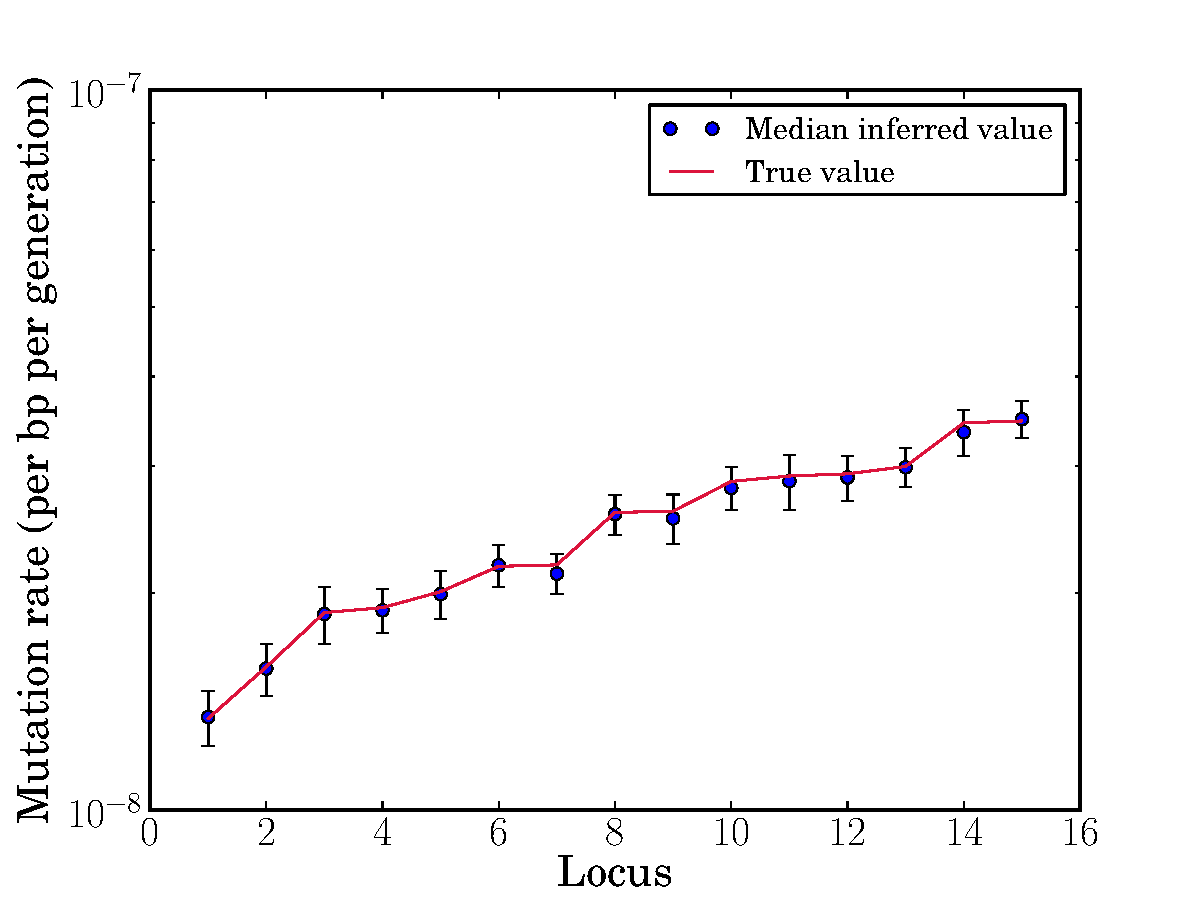
\includegraphics[type=pdf,ext=.pdf,read=.pdf,trim=0 0 0 2cm]{figs/our_method_sdbox_t100_r6.4_rho0.4_maxb18_plotMus}
				%                 %   \label{fig:inferred_mutation_rates}
				%                 %   \caption{
				%                 %   Inferred mutation rates at a random subset of 15 loci for 100 simulated datasets with a recent epoch of exponential growth lasting 100 generations at 6.4\% per generation. The loci are sorted by their true mutation rates.
				%                 %   }
				%                 % \end{figure}
				%                 \end{column}
				% \end{columns}

				
			\end{column}
        	\end{columns}
		\end{block}
		
		\begin{block}{\large Future research directions} \justifying 
			\begin{columns}[T] 
			\begin{column}{.97\linewidth}
			\vspace{-0.7cm}
			\begin{itemize}
				\item Incorporating multiple subpopulations and migration events
				\item Tradeoff in parameter estimation uncertainty as a function of sample size
				\item Model selection
			\end{itemize}
	    	\end{column} 
			\end{columns}
			\vspace{-0.4cm}
		\end{block} 
		
		\begin{block}{\large References} 
			\begin{columns}[T] 
			\begin{column}{.97\linewidth}
			\vspace{-0.8cm}
			\setbeamertemplate{bibliography item}[text]
			\bibliographystyle{myplainnat}
			\scriptsize{\bibliography{../../refs}}
            \vspace{-0.5cm}
			\end{column}
			\end{columns}
		\end{block}
      
	\end{column}
\end{columns}

% TODO: fix alignment of bullet points and text
% TODO: add one more figure or table

% \begin{columns}[t]
%   \begin{column}{.495\linewidth}
%     \end{column}
%     \begin{column}{.495\linewidth}
%     \end{column}
% \end{columns}

	
% \begin{block}{\large Illustration} \Large \justifying \begin{columns}[T] \begin{column}{.96 \linewidth}
% 	Some more testing.
% \end{column} \end{columns} \end{block}
% \vspace{-0.8cm}
% \begin{columns}[T]
% 	\begin{column}{.545\linewidth} 
%        	\begin{block}{\large Background} \justifying \begin{columns}[T] \begin{column}{.96 \linewidth}
% 			Paul and Song.
% 		\end{column} \end{columns} \end{block}
% 		
% 		\begin{block}{\large Results} \justifying \begin{columns}[T] \begin{column}{.96 \linewidth}
% 			We assess
% 		\end{column} \end{columns} \end{block}
% 	\end{column}
% 	\begin{column}{.445\linewidth}
% 		 
%        	\begin{block}{\large Method} \justifying \begin{columns}[T] \begin{column}{.96 \linewidth}
% 			Consider...
% 		\end{column} \end{columns} \end{block}
% 	\end{column}
% \end{columns}

% \begin{columns}[t]
% 	\begin{column}{.495\linewidth} 
% 
% 	\end{column}
% 
%      \begin{column}{.495\linewidth}
%      \end{column}
% \end{columns}

\end{frame}
\end{document}


%%%%%%%%%%%%%%%%%%%%%%%%%%%%%%%%%%%%%%%%%%%%%%%%%%%%%%%%%%%%%%%%%%%%%%%%%%%%%%%%%%%%%%%%%%%%%%%%%%%%
%%% Local Variables: 
%%% mode: latex
%%% TeX-PDF-mode: t
%%% End:
